% Options for packages loaded elsewhere
\PassOptionsToPackage{unicode}{hyperref}
\PassOptionsToPackage{hyphens}{url}
%
\documentclass[
  man,floatsintext]{apa6}
\usepackage{amsmath,amssymb}
\usepackage{lmodern}
\usepackage{iftex}
\ifPDFTeX
  \usepackage[T1]{fontenc}
  \usepackage[utf8]{inputenc}
  \usepackage{textcomp} % provide euro and other symbols
\else % if luatex or xetex
  \usepackage{unicode-math}
  \defaultfontfeatures{Scale=MatchLowercase}
  \defaultfontfeatures[\rmfamily]{Ligatures=TeX,Scale=1}
\fi
% Use upquote if available, for straight quotes in verbatim environments
\IfFileExists{upquote.sty}{\usepackage{upquote}}{}
\IfFileExists{microtype.sty}{% use microtype if available
  \usepackage[]{microtype}
  \UseMicrotypeSet[protrusion]{basicmath} % disable protrusion for tt fonts
}{}
\makeatletter
\@ifundefined{KOMAClassName}{% if non-KOMA class
  \IfFileExists{parskip.sty}{%
    \usepackage{parskip}
  }{% else
    \setlength{\parindent}{0pt}
    \setlength{\parskip}{6pt plus 2pt minus 1pt}}
}{% if KOMA class
  \KOMAoptions{parskip=half}}
\makeatother
\usepackage{xcolor}
\usepackage{graphicx}
\makeatletter
\def\maxwidth{\ifdim\Gin@nat@width>\linewidth\linewidth\else\Gin@nat@width\fi}
\def\maxheight{\ifdim\Gin@nat@height>\textheight\textheight\else\Gin@nat@height\fi}
\makeatother
% Scale images if necessary, so that they will not overflow the page
% margins by default, and it is still possible to overwrite the defaults
% using explicit options in \includegraphics[width, height, ...]{}
\setkeys{Gin}{width=\maxwidth,height=\maxheight,keepaspectratio}
% Set default figure placement to htbp
\makeatletter
\def\fps@figure{htbp}
\makeatother
\setlength{\emergencystretch}{3em} % prevent overfull lines
\providecommand{\tightlist}{%
  \setlength{\itemsep}{0pt}\setlength{\parskip}{0pt}}
\setcounter{secnumdepth}{-\maxdimen} % remove section numbering
% Make \paragraph and \subparagraph free-standing
\ifx\paragraph\undefined\else
  \let\oldparagraph\paragraph
  \renewcommand{\paragraph}[1]{\oldparagraph{#1}\mbox{}}
\fi
\ifx\subparagraph\undefined\else
  \let\oldsubparagraph\subparagraph
  \renewcommand{\subparagraph}[1]{\oldsubparagraph{#1}\mbox{}}
\fi
\newlength{\cslhangindent}
\setlength{\cslhangindent}{1.5em}
\newlength{\csllabelwidth}
\setlength{\csllabelwidth}{3em}
\newlength{\cslentryspacingunit} % times entry-spacing
\setlength{\cslentryspacingunit}{\parskip}
\newenvironment{CSLReferences}[2] % #1 hanging-ident, #2 entry spacing
 {% don't indent paragraphs
  \setlength{\parindent}{0pt}
  % turn on hanging indent if param 1 is 1
  \ifodd #1
  \let\oldpar\par
  \def\par{\hangindent=\cslhangindent\oldpar}
  \fi
  % set entry spacing
  \setlength{\parskip}{#2\cslentryspacingunit}
 }%
 {}
\usepackage{calc}
\newcommand{\CSLBlock}[1]{#1\hfill\break}
\newcommand{\CSLLeftMargin}[1]{\parbox[t]{\csllabelwidth}{#1}}
\newcommand{\CSLRightInline}[1]{\parbox[t]{\linewidth - \csllabelwidth}{#1}\break}
\newcommand{\CSLIndent}[1]{\hspace{\cslhangindent}#1}
\ifLuaTeX
\usepackage[bidi=basic]{babel}
\else
\usepackage[bidi=default]{babel}
\fi
\babelprovide[main,import]{english}
% get rid of language-specific shorthands (see #6817):
\let\LanguageShortHands\languageshorthands
\def\languageshorthands#1{}
% Manuscript styling
\usepackage{upgreek}
\captionsetup{font=singlespacing,justification=justified}

% Table formatting
\usepackage{longtable}
\usepackage{lscape}
% \usepackage[counterclockwise]{rotating}   % Landscape page setup for large tables
\usepackage{multirow}		% Table styling
\usepackage{tabularx}		% Control Column width
\usepackage[flushleft]{threeparttable}	% Allows for three part tables with a specified notes section
\usepackage{threeparttablex}            % Lets threeparttable work with longtable

% Create new environments so endfloat can handle them
% \newenvironment{ltable}
%   {\begin{landscape}\centering\begin{threeparttable}}
%   {\end{threeparttable}\end{landscape}}
\newenvironment{lltable}{\begin{landscape}\centering\begin{ThreePartTable}}{\end{ThreePartTable}\end{landscape}}

% Enables adjusting longtable caption width to table width
% Solution found at http://golatex.de/longtable-mit-caption-so-breit-wie-die-tabelle-t15767.html
\makeatletter
\newcommand\LastLTentrywidth{1em}
\newlength\longtablewidth
\setlength{\longtablewidth}{1in}
\newcommand{\getlongtablewidth}{\begingroup \ifcsname LT@\roman{LT@tables}\endcsname \global\longtablewidth=0pt \renewcommand{\LT@entry}[2]{\global\advance\longtablewidth by ##2\relax\gdef\LastLTentrywidth{##2}}\@nameuse{LT@\roman{LT@tables}} \fi \endgroup}

% \setlength{\parindent}{0.5in}
% \setlength{\parskip}{0pt plus 0pt minus 0pt}

% Overwrite redefinition of paragraph and subparagraph by the default LaTeX template
% See https://github.com/crsh/papaja/issues/292
\makeatletter
\renewcommand{\paragraph}{\@startsection{paragraph}{4}{\parindent}%
  {0\baselineskip \@plus 0.2ex \@minus 0.2ex}%
  {-1em}%
  {\normalfont\normalsize\bfseries\itshape\typesectitle}}

\renewcommand{\subparagraph}[1]{\@startsection{subparagraph}{5}{1em}%
  {0\baselineskip \@plus 0.2ex \@minus 0.2ex}%
  {-\z@\relax}%
  {\normalfont\normalsize\itshape\hspace{\parindent}{#1}\textit{\addperi}}{\relax}}
\makeatother

% \usepackage{etoolbox}
\makeatletter
\patchcmd{\HyOrg@maketitle}
  {\section{\normalfont\normalsize\abstractname}}
  {\section*{\normalfont\normalsize\abstractname}}
  {}{\typeout{Failed to patch abstract.}}
\patchcmd{\HyOrg@maketitle}
  {\section{\protect\normalfont{\@title}}}
  {\section*{\protect\normalfont{\@title}}}
  {}{\typeout{Failed to patch title.}}
\makeatother

\usepackage{xpatch}
\makeatletter
\xapptocmd\appendix
  {\xapptocmd\section
    {\addcontentsline{toc}{section}{\appendixname\ifoneappendix\else~\theappendix\fi\\: #1}}
    {}{\InnerPatchFailed}%
  }
{}{\PatchFailed}
\keywords{emotion regulation, regulatory effort, effort discounting, registered report, specification curve analysis\newline\indent Word count: 6289}
\usepackage{csquotes}
\usepackage{booktabs}
\usepackage{longtable}
\usepackage{array}
\usepackage{multirow}
\usepackage{wrapfig}
\usepackage{float}
\usepackage{colortbl}
\usepackage{pdflscape}
\usepackage{tabu}
\usepackage{threeparttable}
\usepackage{threeparttablex}
\usepackage[normalem]{ulem}
\usepackage{makecell}
\usepackage{xcolor}
\usepackage{setspace}\doublespacing
\usepackage[final]{pdfpages}
\usepackage{chngcntr}
\ifLuaTeX
  \usepackage{selnolig}  % disable illegal ligatures
\fi
\IfFileExists{bookmark.sty}{\usepackage{bookmark}}{\usepackage{hyperref}}
\IfFileExists{xurl.sty}{\usepackage{xurl}}{} % add URL line breaks if available
\urlstyle{same} % disable monospaced font for URLs
\hypersetup{
  pdftitle={Estimating individual subjective values of emotion regulation strategies},
  pdfauthor={Christoph Scheffel,1, Josephine Zerna,1, Anne Gärtner1, Denise Dörfel1, \& Alexander Strobel1},
  pdflang={en-EN},
  pdfkeywords={emotion regulation, regulatory effort, effort discounting, registered report, specification curve analysis},
  hidelinks,
  pdfcreator={LaTeX via pandoc}}

\title{Estimating individual subjective values of emotion regulation strategies}
\author{Christoph Scheffel\textsuperscript{$\dagger{}$,1}, Josephine Zerna\textsuperscript{$\dagger{}$,1}, Anne Gärtner\textsuperscript{1}, Denise Dörfel\textsuperscript{1}, \& Alexander Strobel\textsuperscript{1}}
\date{}


\shorttitle{Subjective values of emotion regulation strategies}

\authornote{

The authors made the following contributions. Christoph Scheffel: Conceptualization, Methodology, Funding acquisition, Formal analysis, Investigation, Project administration, Software, Visualization, Writing - original draft preparation, Writing - review \& editing; Josephine Zerna: Conceptualization, Methodology, Funding acquisition, Investigation, Project administration, Software, Visualization, Writing - review \& editing; Anne Gärtner: Formal analysis, Writing - review \& editing; Denise Dörfel: Conceptuatlization, Writing - review \& editing; Alexander Strobel: Conceptualization, Writing - review \& editing. \textsuperscript{$\dagger{}$} Christoph Scheffel and Josephine Zerna contributed equally to this work.

Correspondence concerning this article should be addressed to Christoph Scheffel, Zellescher Weg 17, 01069 Dresden, Germany. E-mail: \href{mailto:christoph_scheffel@tu-dresden.de}{\nolinkurl{christoph\_scheffel@tu-dresden.de}}

}

\affiliation{\vspace{0.5cm}\textsuperscript{1} Faculty of Psychology, Technische Universität Dresden, 01069 Dresden, Germany}

\abstract{%
Individuals have a repertoire of emotion regulation (ER) strategies at their disposal, which they can use more or less flexibly.
In ER flexibility research, strategies that facilitate goal achievement are considered adaptive and therefore are subjectively valuable.
Individuals are motivated to reduce their emotional arousal effectively and to avoid cognitive effort.
Perceived costs of ER strategies in the form of effort, however, are highly subjective.
Subjective values (SVs) should therefore represent a trade-off between effectiveness and subjectively required cognitive effort.
However, SVs of ER strategies have not been determined so far.
We present a paradigm that is suitable for determining individual SVs of ER strategies.
Using a multilevel modelling approach, it will be investigated whether individual SVs can be explained by effectiveness (subjective arousal, facial muscle activity) and subjective effort.
Relations of SVs to personality traits will be explored.
}



\begin{document}
\maketitle

\renewcommand\thesection{\Alph{section}}
\counterwithout{figure}{section}
\setcounter{figure}{0}

\begin{center}\rule{0.5\linewidth}{0.5pt}\end{center}

\hypertarget{introduction}{%
\section{1. Introduction}\label{introduction}}

The ability to modify emotional experiences, expressions, and physiological reactions\textsuperscript{1} to regulate emotions is an important cognitive skill.
It is therefore not surprising that emotion regulation (ER) has substantial implications for well-being and adaptive functioning\textsuperscript{2}.
Different strategies can be used to regulate emotions, namely situation selection, situation modification, attentional deployment, cognitive change, and response modification\textsuperscript{1}, and, following the taxonomy of Powers and LaBar\textsuperscript{3}, individuals can implement ER strategies by means of different tactics.
So called antecedent-focused strategies, e.g., attentional deployment and cognitive change, take effect early in the emotion generation process\textsuperscript{1}.
In contrast, response modification takes place late in the process and is therefore conceptualized as a response-focused strategy\textsuperscript{1}.
This postulated temporal sequence of ER strategies influences their effectiveness.
Albeit it is meta-analytically proven that all mentioned strategies reduce subjective emotional experience, distraction as a tactic of attentional deployment and (expressive) suppression as a tactic of response modulation showed only small to medium effect sizes (distraction: \emph{d\textsubscript{+}} = 0.27; suppression: \emph{d\textsubscript{+}} = 0.27).
In contrast, distancing as tactic of cognitive change showed the highest effectiveness with an effect size of \emph{d\textsubscript{+}} = 0.45\textsuperscript{4}.

Psychophysiological measures provide further important information on the effectiveness of emotion regulation strategies (for an overview, see Zaehringer et al.\textsuperscript{5}).
Compared to cardiovascular, electrodermal, and pupillometric autonomic responses, facial electromyography has been reported consistently across studies to be influenced by emotion regulation with even medium effect sizes.
For example, studies have shown that reappraisal of negative emotion is associated with reduced activity of the corrugator supercilii (associated with anger, sadness, and fear) with \emph{d\textsubscript{-}} = 0.32\textsuperscript{5}.
In addition, the levator labii superioris (associated with disgust) has also been associated with reduced activity during reappraisal\textsuperscript{6}.
Similar effects have been reported for suppression\textsuperscript{6}, distancing\textsuperscript{7}, and distraction\textsuperscript{8}.
Importantly, results on electromyographic measures seem to be more consistent compared to other autonomic measures, likely because they are specific to emotional valence and its changes.

Similarly to the differences in short term effectiveness, these tactics from three different strategies are also related to different medium and long-term consequences.
In particular, strategies that do not change the emotional content of the situation, for instance by taking a neutral perspective (i.e., distraction and suppression) are presumed to be disadvantageous in the longer term.
Thus, the self-reported habitual use of suppression is associated with more negative affect and lower general well-being\textsuperscript{9}.
In addition, a number of ER strategies, e.g., rumination and suppression, have been associated with mental disorders (for meta-analytic review, see Aldao et al.\textsuperscript{10}), which led to the postulation of \emph{adaptive} (such as reappraisal, acceptance) and \emph{maladaptive} (such as suppression, rumination) ER strategies.
For example, it was shown that maladaptive ER strategies (rumination and suppression) mediate the effect between neuroticism and depressive symptoms\textsuperscript{11}.

The postulation of \emph{adaptive} and \emph{maladaptive} ER strategies has been challenged by the concepts of ER repertoire and ER flexibility.
Within this framework, \emph{maladaptive} refers to inflexible ER strategy use or use of strategies that are hindering goal achievement\textsuperscript{12}.
Adaptive flexible ER requires a large repertoire of ER strategies\textsuperscript{12}.
The term ``repertoire'' can be defined as the ability to utilize a wide range of regulatory strategies in divergent contextual demands and opportunities\textsuperscript{13}.
A growing number of studies report findings about the repertoire of emotion regulation strategies and its relationship to psychopathology\textsuperscript{14--16}.
Additionally, greater ER flexibility is related to reduced negative affect and therefore beneficial in daily life\textsuperscript{17}.

How do people choose strategies from their repertoire?
Similarly to the expectancy-value model of emotion regulation\textsuperscript{18} it could be assumed, that people also assign a value to an ER strategy reflecting the usefulness of this strategy for goal achieving.
Evidence from other psychological domains (e.g., intertemporal choice\textsuperscript{19}) shows that subjective values (SVs) are attributed to the choice options on the basis of which the decision is made.
Research on ER choice has identified numerous factors that influence the choice of ER strategies, which can be seen as indirect evidence for factors influencing SVs\textsuperscript{20}.
For example, a study found that the intensity of a stimulus or situation plays a role in the choice\textsuperscript{21}.
Higher intensity of the (negative) stimulus lead to a choice of rather disengaging tactics of attentional deployment, like distraction\textsuperscript{20,21}.
ER choice was further influenced by, among others, extrinsic motivation (e.g., monetary incentives), motivational determinants (i.e., hedonic regulatory goals), and effort\textsuperscript{20,22}.
Nonetheless, there are only few studies to date that examined the required effort of several strategies in more detail and compared them with each other.
Furthermore, the research on ER choice lacks information regarding the strategies that were \emph{not} chosen in each case.
It is unclear whether people had clear preferences or whether the choice options were similarly attractive.

We assume that people choose the strategy that has the highest value for them at the moment.
The value is determined against the background of goal achievement in the specific situation: A strategy is highly valued if it facilitates goal achievement\textsuperscript{12}.
One certainly central goal is the regulation of negative affect.
The effectiveness of ER strategies should therefore influence the respective SV.
A second, intrinsic, and less obvious goal is the avoidance of effort\textsuperscript{23}.
When given the choice, most individuals prefer tasks that are less effortful\textsuperscript{24}.
Cognitive effort avoidance has been reported in many contexts, for example in affective context\textsuperscript{25}, the context of decision making\textsuperscript{26}, and executive functions\textsuperscript{27}, and is associated with Need for Cognition (NFC)\textsuperscript{28}, a stable measure of the individual pursuit and enjoyment of cognitive effort\textsuperscript{29,30}.
In the area of emotion regulation, too, there are initial indications that people show a tendency towards effort avoidance.
Across two studies, we could show in previous work that the choice for an ER strategy is mainly influenced by the effort required to implement a given strategy\textsuperscript{22}.
In our studies, participants used the strategies distancing and suppression while inspecting emotional pictures.
Afterwards, they choose which strategy they wanted to use again.
Participants tended to re-apply the strategy that was subjectively less effortful, even though it was subjectively not the most effective one - in this case: suppression.
Moreover, the majority of participants stated afterwards the main reason for their choice was effort.
We assume therefore that, although individuals trade off both factors - effectiveness and effort - against each other, effort should be the more important predictor for SVs of ER strategies.
In addition, perceived utility should have an impact on SVs.
A strategy that is less effortful and can objectively regulate arousal (i.e., is effective), but is not subjectively perceived as useful, should have a low SV.
SVs of ER Strategies could therefore be helpful to describe the ER repertoire\textsuperscript{12} more comprehensively.
Depending on the flexibility of a person, different patterns of SVs could be conceivable: A person with high flexibility would show relatively high SVs for a number of strategies.
This would mean that all strategies are a good option for goal achievement.
A second person with less flexibility, however, would show high SVs only for one strategy or low SVs for all of the strategies.
This in turn would mean that there is only a limited amount of strategies in the repertoire to choose from.
Subsequently, the ability to choose an appropriate strategy for a specific situation is also limited.

So far we have not seen any attempt in ER choice research to determine individual SVs of ER strategies.
However, this would be useful to describe interindividual differences in the preference of ER strategies and the ER repertoire more comprehensively.
To investigate this question, the individual SVs of each strategy available for selection would have to be determined.
Promising approaches can be found in studies on difficulty levels of effortful cognitive tasks.\\
Individual SVs of effortful cognitive tasks have been quantified using the Cognitive Effort Discounting Paradigm (COG-ED)\textsuperscript{29}.

In the original study by Westbrook et al.\textsuperscript{29}, cognitive load was varied using the \emph{n}-back task, a working memory task that requires fast and accurate responses to sequentially presented stimuli.
Participants had to decide in an iterative procedure whether they wanted to repeat a higher \emph{n}-back level for a larger, fixed monetary reward, or a lower level for a smaller, varying reward, with the implicit assumption that the objectively easiest \emph{n}-back level has the highest SV.
In the present study, we want to use this paradigm to determine SVs of ER strategies.
In doing so, we need to make an important change: We have to adapt the assumption that the easiest \emph{n}-back level has the highest SV.
As we have shown in previous studies, there are large inter-individual differences in the preference and perceived subjective effort of ER strategies\textsuperscript{22}.
Moreover, there is nothing like an objectively easiest ER strategy.
It could be assumed, that the antecedent-focused strategies, i.e.~attentional deployment and cognitive change, require less effort, because according to Gross\textsuperscript{1} these strategies apply when the emotional reaction has not fully developed, yet.
In contrast, suppression would need ongoing effort, because it takes effect late in the emotion generating process and does not alter the emotion itself.
A similar assumption has been made by Mesmer-Magnus et al.\textsuperscript{31}, who state that Surface Acting (the equivalent to expressive suppression in emotional labor research) is supposed to continuously require high levels of energy (hence effort).
Deep Acting (which refers to reappraisal), in turn, only initially needs the use of energy.
This would be in conflict with findings in our previous studies, that showed that many people choose expressive suppression because they evaluated it as less effortful, hence easy\textsuperscript{22}.
Others define emotion regulation on a continuum from explicit, conscious, and effortful to implicit, unconscious, automatic and effortless\textsuperscript{32}.
This would mean, that all explicit strategies that have been proposed by the process model of emotion regulation are similarly effortful\textsuperscript{1}.
Similarly, the flexibility approach of emotion regulation also states, that there is no ``best'' strategy\textsuperscript{33}.
An emotion regulation attempt is adaptive, when the intended, individual goal is reached. Those attempts could also consist of sequences of regulatory efforts using different strategies, which might be effective and effortless only in this specific context.
Therefore, we have to add an additional step, which precedes the other steps and where the ER option with the higher subjective value is determined.
In this step, the same monetary value (i.e., 1 €) is assigned to both options.
The assumption is that participants now choose the option that has the higher SV for them.
In the next step we return to the original paradigm.
The higher monetary value (i.e., 2 €) is assigned to the option that was not chosen in the first step and therefore is assumed to have the lower SV.
In the following steps, the lower value is changed in every iteration according to Westbrook et al.\textsuperscript{29} until the indifference point is reached.
This procedure will be repeated until all strategies have been compared.
The SV of each strategy is calculated as the mean of this strategy's SV from all comparisons.
In case a participant has a clear preference for one strategy, the SV of this strategy will be 1.
But our paradigm can also account for the case that a person does not have a clear preference.
Then no SV will be 1, but still, the SVs of all strategies can be interpreted as absolute values and in relation to the other strategy's SVs (see Figure 1).
In a separate study, we will test our adapted paradigm together with a \emph{n}-back task and explore whether this paradigm can describe individuals that do not prefer the easiest \emph{n}-back option (see Zerna et al.\textsuperscript{34}).

INSERT FIGURE 1 HERE

The aim of the present study is to evaluate whether this paradigm is suitable for determining SVs of ER strategies.
As a manipulation check, we first want to investigate whether the valence of the pictures is affecting subjective and physiological responding, resulting in lower subjective arousal ratings after and lower EMG activity during neutral compared to negative pictures.
Second, we want to check whether the ER strategies distraction, distancing, and suppression effectively reduce subjective arousal and physiological responding compared to the active viewing condition.
Third, we want to see whether the strategies subjectively require more cognitive effort than the active viewing condition, and whether participants re-apply the for them least effortful strategy.
Furthermore, we want to investigate whether subjective effort, arousal ratings, subjective utility, and EMG activity predict individual subjective values of ER strategies.
And lastly, we want to check whether the SV of a strategy is associated with its likelihood of being chosen again, and whether SVs reflect participants' self-reported ER flexibility.
All hypotheses are detailed in the \protect\hyperlink{DesignTable}{design table}.
Exploratorily, we want to investigate whether individual SVs are related to personality traits and how individual SVs of ER strategies relate to SVs of other tasks with different demand levels, namely \emph{n}-back.

\hypertarget{method}{%
\section{2. Method}\label{method}}

We report how we determined our sample size, all data exclusions (if any), all manipulations, and all measures in the study\textsuperscript{35}.
The paradigm was written and presented using \emph{PsychoPy}\textsuperscript{36}.
We used \emph{R} with \emph{R Studio}\textsuperscript{37,38} with the main packages \emph{afex}\textsuperscript{39} and \emph{BayesFactor}\textsuperscript{40} for all analyses.
The R Markdown file used to analyze the data and write this document, as well as the raw data and the materials are freely available at \url{https://github.com/ChScheffel/CAD}.
A complete list of all measures assessed in the study can be found at OSF (\url{https://osf.io/vnj8x/}) and GitHub (\url{https://github.com/ChScheffel/CAD}).

\hypertarget{ethics-information}{%
\subsection{2.1 Ethics information}\label{ethics-information}}

The study protocol complies with all relevant ethical regulations and was approved by the ethics committee of the Technische Universität Dresden (reference number EK50012022).
Prior to testing, written informed consent will be obtained.
Participants will receive 30 € in total or course credit for participation.

\hypertarget{pilot-data}{%
\subsection{2.2 Pilot data}\label{pilot-data}}

The newly developed ER paradigm was tested in a pilot study with \(N=16\) participants (9 female; age: \(M = 24.1\text{ }\pm\text{ }SD = 3.6\)).
Regarding self-reported arousal, results showed significant higher subjective arousal for active viewing of negative compared to neutral pictures.
However, ER strategies did not lead to a reduction of subjective arousal compared to active viewing of negative pictures.
Regarding physiological responses, ER strategies were associated with reduced facial muscle activity of the \emph{corrugator} and \emph{levator} compared to active viewing of negative pictures.
In accordance with our previous study\textsuperscript{22}, we found that the use of ER strategies compared to active viewing was associated with increased subjective effort.
All results are detailed in the \protect\hyperlink{SupplementaryMaterial}{Supplementary Material}, figures S1 to S7 and table S2 to S8.

\hypertarget{design}{%
\subsection{2.3 Design}\label{design}}

Young healthy participants (aged 18 to 30 years) will be recruited using the software \emph{ORSEE}\textsuperscript{41} at the Technische Universität Dresden.
Participants will be excluded from participation if they do not fluently speak German, have current or a history of psychological disorders or neurological trauma, or report to take medication.
Participants will be invited to complete an online survey containing different questionnaires to assess broad and narrow personality traits and measures of well-being.
The study consists of two lab sessions, which will take place in a shielded cabin with constant lighting.
Before each session, participants will receive information about the respective experimental procedure and provide informed consent.
In the first session participants will fill out a demographic questionnaire and complete an n-back task with the levels one to four.
Then, they will complete an effort discounting (ED) procedure regarding the n-back levels on screen, followed by a random repetition of one n-back level.
The second session will take place exactly one week after session one.
Participants will provide informed consent and receive written instructions on the ER paradigm and ER strategies that they should apply.
A brief training will ensure that all participants are able to implement the ER strategies.
Next, electrodes to measure facial EMG will be attached and the ER task will be conducted, followed by an ED procedure regarding the ER strategies.
After that, participants will choose one ER strategy to repeat one more time.
Study data will be collected and managed using REDCap electronic data capture tools hosted at Technische Universität Dresden\textsuperscript{42,43}.

\hypertarget{psychometric-measures}{%
\subsubsection{2.3.1 Psychometric measures}\label{psychometric-measures}}

The online survey will contain a number of questionnaires.
In the focus of the current project is the Flexible Emotion Regulation Scale (FlexER)\textsuperscript{44}.\\
It assesses flexible use of ER strategies with items such as ``If I want to feel less negative emotions, I have several strategies to achieve this.'', which we define as ER flexibility.
The items are rated on a 4-point scale ranging from ``strongly agree'' to ``strongly disagree''.

Further psychological constructs will be assessed but have no clear hypotheses in the present work and are therefore investigated only exploratory:
General psychological well-being will be assessed using the German version of the WHO-5 scale\textsuperscript{45,46}.
To measure resilience, the German version 10-item-form of the Connor-Davidson resilience Scale (CD-RISC)\textsuperscript{49} will be used.
Habitual use of ER will be assessed using the German version of the Emotion Regulation Questionnaire (ERQ)\textsuperscript{9,50}.
Implicit theories of willpower in emotion control will be assessed using the implicit theories questionnaire from Bernecker and Job\textsuperscript{51}.
To assess Need for Cognition, the German version short form of the Need for Cognition Scale\textsuperscript{28,52} will be used.
To assess self-control\textsuperscript{53}, sum scores of the German versions of the following questionnaires will be used: the Self-Regulation Scale (SRS)\textsuperscript{54}, the Brief Self-Control Scale (BSCS)\textsuperscript{55,56}, and the Barratt Impulsiveness Scale (BIS-11)\textsuperscript{57,58}.
Attentional control will be assessed using the Attentional Control Scale (ACS)\textsuperscript{59}.
For more detailed information on psychometric properties of the questionnaires, please see \protect\hyperlink{SupplementQuestionnaires}{supplementary material}.

\hypertarget{emotion-regulation-paradigm}{%
\subsubsection{2.3.2 Emotion regulation paradigm}\label{emotion-regulation-paradigm}}

The ER paradigm will consist of three parts that will be described in the following.

\emph{Part one: ER task.} Part one will be a standard ER task in a block design (see Figure 2), similar to paradigms previously used by our group\textsuperscript{22}.
Participants will be told to actively view neutral and negative pictures (see \protect\hyperlink{ux5cux23stimuli}{2.3.3}) or to regulate all upcoming emotions by means of distraction, distancing, and expressive suppression, respectively.
Every participant first will have the condition ``active viewing-neutral'' that serves as a baseline condition.
During this block, 20 neutral pictures will be presented.
Participants will be asked to ``actively view all pictures and permit all emotions that may arise.''
In the second block, participants will actively view negative pictures.
During the third, fourth, and fifth block, participants will see negative pictures and will be asked to regulate their emotions using distraction, distancing, and suppression.
In order to achieve distraction, participants will be asked to think of a geometric object or an everyday activity, like brushing their teeth.
During distancing, participants will be asked to ``take the position of a non-involved observer, thinking about the picture in a neutral way.''
Participants will be told not to re-interpret the situation or attaching a different meaning to the situation.
During suppression, participants will be told to ``suppress their emotional facial expression.''
They should imagine being observed by a third person that should not be able to tell by looking at the facial expression whether the person is looking at an emotional picture.
Participants will be instructed not to suppress their thoughts or change their facial expression to the opposite\textsuperscript{22}.
All participants will receive written instruction and complete a training session.
After the training session, participants will be asked about their applied ER strategies to avoid misapplication.
The order of the three regulation blocks (distraction, distancing, and suppression) will be randomized between participants.
Each of the blocks consists of 20 trials showing neutral (Block 1) and negative (Blocks 2, 3, 4, 5) pictures.
Each trial begins with a fixation cross that lasts 3 to 5 seconds (random uniform distributed).
It is followed by neutral or negative pictures for a total of 6 seconds.
After each block, participants retrospectively will rate their subjective emotional arousal (``not at all aroused'' to ``very highly aroused''), their subjective effort (``not very exhausting'' to ``very exhausting''), and - after the ragulation blocks - the utility of the respective strategy (``not useful at all'' to ``very useful'') on a continuous scale using a slider on screen.

\emph{Part two: ER effort discounting.} In the second part, ER effort discounting will take place.
The procedure of the discounting will follow the COG-ED paradigm by Westbrook et al.\textsuperscript{29} with a major change.
We will use the following adaption that allows the computation of SVs for different strategies without presuming that all individuals would inherently evaluate the same strategy as the easiest one: For each possible pairing (distraction vs.~distancing, distraction vs.~suppression, and distancing vs.~suppression), each of the two strategies will be presented with a monetary reward.
Because there is no strategy that is objectively more difficult, we will add initial comparisons asking the participants to choose between ``1 € for strategy A or 1 € for strategy B''.
They decide by clicking the on-screen button of the respective option.
Each of the three strategy pairs will be presented three times in total, in a randomized order and randomly assigned which strategy appears on the left or right side of the screen.
For each pair, the strategy that was chosen at least two out of three times will be assigned the flexible starting value of 1 €, the other strategy will be assigned the fixed value of 2 €.
After this, comparisons between strategies will follow the original COG-ED paradigm\textsuperscript{29}.
Each pairing is presented six consecutive times, and with each decision the reward of the strategy with the starting value of 1 € is either lowered (if this strategy was chosen) or raised (if the strategy with the fixed 2 € reward was chosen).
The adjustment starts at 0.50 € and each is half the adjustment of the previous step, rounded to two digits after the decimal point.
If a participant always chooses the strategy with the fixed 2 € reward, the other strategy's last value on display will be 1.97 €, if they always choose the lower strategy, its last value will be 0.03 €.
The sixth adjustment of 0.02 € will be done during data analysis, based on the participants' decision in the last display of the pairing.
Participants will be instructed to decide as realistically as possible by imagining that the monetary reward is actually available for choice.

\emph{Part three: ER choice.} After the discounting part, participants will choose which one of the three ER strategies (distraction, distancing or suppression) they want to re-apply.
Importantly, there will be no further instruction on what basis they should make their decision.
Participants should make their decision freely, according to criteria they consider important for themselves.
However, participants will be asked to state the reasons for the decision afterwards in RedCap using a free text field.
As soon as they have decided, they will see the respective instruction and the block with another 20 negative pictures starts.

INSERT FIGURE 2 HERE

\hypertarget{stimuli}{%
\subsubsection{2.3.3 Stimuli}\label{stimuli}}

Pictures that will be used in the paradigm are selected from the Emotional Picture Set (EmoPicS)\textsuperscript{60} and the International Affective Picture System (IAPS)\textsuperscript{61}.
The 20 neutral pictures (Valence (V): \emph{M} \(\pm\) \emph{SD} = 4.81 \(\pm\) 0.51; Arousal (A): \emph{M} \(\pm\) \emph{SD} = 3 \(\pm\) 0.65) depicted content related to the categories persons, objects, and scenes.
Further, 100 negative pictures, featuring categories animals, body, disaster, disgust, injury, suffering, violence, and weapons, will be used.
An evolutionary algorithm\textsuperscript{62} is used to cluster these pictures into five sets with comparable valence and arousal values (set one: V: \emph{M} \(\pm\) \emph{SD} = 2.84 \(\pm\) 0.57, A: \emph{M} \(\pm\) \emph{SD} = 5.62 \(\pm\) 0.34; set two: V: \emph{M} \(\pm\) \emph{SD} = 2.64 \(\pm\) 0.46, A: \emph{M} \(\pm\) \emph{SD} = 5.58 \(\pm\) 0.35; set three: V: \emph{M} \(\pm\) \emph{SD} = 2.82 \(\pm\) 0.62, A: \emph{M} \(\pm\) \emph{SD} = 5.60 \(\pm\) 0.39; set four: V: \emph{M} \(\pm\) \emph{SD} = 2.65 \(\pm\) 0.75, A: \emph{M} \(\pm\) \emph{SD} = 5.61 \(\pm\) 0.41; set five: V: \emph{M} \(\pm\) \emph{SD} = 2.74 \(\pm\) 0.70, A: \emph{M} \(\pm\) \emph{SD} = 5.63 \(\pm\) 0.37).
A complete list of all pictures and their classification into sets can be found in supplementary material table S1.
The five sets of negative pictures will be assigned randomly to the blocks.

\hypertarget{facial-electromyography}{%
\subsubsection{2.3.4 Facial electromyography}\label{facial-electromyography}}

Bipolar facial electromyography (EMG) will be measured for \emph{corrugator supercilii} and \emph{levator labii} as indices of affective valence\textsuperscript{63}, similar to previous work by our group\textsuperscript{7}.
Two passive surface Ag/AgCl electrodes (8 mm inner diameter, 10 mm distance between electrodes) will be placed over each left muscle according to the guidelines of\textsuperscript{64}.
The ground electrode will be placed over the left \emph{Mastoid}.
Before electrode placement, the skin will be abraded with Every abrasive paste, cleaned with alcohol, and filled with Lectron III electrolyte gel.
Raw signals will be amplified by a BrainAmp amplifier (Brain Products Inc., Gilching, Germany).
Impedance level will be kept below 10 \(k\Omega\).
Data will be sampled at 1000 Hz, filtered, rectified and integrated.
A 20 Hz high pass (order 8), a 300 Hz low pass (order 8), and a 50 Hz notch filter will be applied to both signals.
Corrugator and Levator EMG will be analyzed during the 6 s of picture presentation.
EMG data will be baseline-corrected using a time window of 2 s prior to stimulus onset\textsuperscript{63}.
Last, the sampling rate will be changed to 100 Hz, and EMG data will be averaged for each condition and each participant.

\hypertarget{sampling-plan}{%
\subsection{2.4 Sampling plan}\label{sampling-plan}}

Sample size calculation is done using \emph{G*Power}\textsuperscript{65,66}.
In a meta-analysis of Zaehringer and colleagues\textsuperscript{5}, effect sizes of ER on peripheral-physiological measures were reported:
To find an effect of \(d=-0.32\) of ER on \emph{corrugator} muscle activity with \(\alpha=.05\) and \(\beta=.95\), data of at least \(N=85\) have to be analyzed.
Power analyses of all other hypotheses yielded smaller sample sizes.
However, if participants withdraw from study participation, technical failures occur, or experimenter considers the participant for not suitable for study participation (e.g., because the participant does not follow instructions or shows great fatigue), respective data will also be excluded from further analyses.
Therefore, we aim to collect data of \(N=120\) participants, about \(50%
\) more data sets, than necessary.
Detailed information on power calculation for each hypothesis can be found in the \protect\hyperlink{DesignTable}{design table}.

\hypertarget{analysis-plan}{%
\subsection{2.5 Analysis plan}\label{analysis-plan}}

Data collection and analysis will not be performed blind to the conditions of the experiments.
Data of whole participants will be excluded from analysis if participants withdraw their consent or they state that they did not follow experimental instructions.
EMG data of subjects will be excluded from analysis if errors occured during recording.
No further data exclusions are planned.
The level of significance will be set to \(\alpha=.05\).
For hypotheses H1-4, repeated measures analysis of variance (rmANOVA) will be conducted and estimated marginal means will be computed using the \emph{afex} package\textsuperscript{39}.
Greenhouse-Geisser-corrected degrees of freedom and associated \(p\)-values will be reported when the assumption of sphericity is violated.
If the within-subjects factor of interest is significant, pairwise contrasts will be calculated using Bonferroni adjustment for multiple testing.
Proportion of explained variance \(\eta_{p}^{2}\) will be reported as a measure of effect size.

\emph{Effect of valence on arousal and facial EMG.}
To examine the impact of valence of emotional pictures on subjective arousal ratings (H1a), a rmANOVA with the factor valence (neutral and negative) for the strategy active viewing will be conducted.
To examine the impact of valence on physiolocigal responding (H1b and H1c), a rmANOVA with the factor valence (neutral and negative) for the strategy active viewing will be conducted for EMG \emph{corrugator} and \emph{levator} activity.

\emph{Effects of emotion regulation on arousal, facial EMG and effort.}
To investigate the effects of the three ER strategies on subjective arousal (H2a), another rmANOVA with the factor strategy (active viewing - negative, distraction, distancing, and suppression) for subjective arousal ratings will be conducted.
To examine the effects of the three ER strategies on physiological responding (H3a and H3b), another rmANOVA with the factor strategy (active viewing - negative, distraction, distancing, and suppression) for EMG \emph{corrugator} and \emph{levator} activity will be conducted.
To examine the effect of ER strategies on subjective effort (H4a), a rmANOVA with the factor strategy (active viewing - negative, distraction, distancing, and suppression) for subjective effort ratings will be conducted.

\emph{Subjective values of emotion regulation strategies.} For each ER strategy, SVs will be calculated as follows: first, the value 0.02 € will be added to or subtracted from the last monetary value of the flexible strategy, depending on the participant's last choice.
Second, to obtain the SV of the fixed strategy (the minimum relative reward required for participants to choose the flexible over the fixed strategy), the last value of the flexible strategy will be divided by 2 €.
Therefore, the SVs of the flexible strategies are 1, because they were chosen in the initial comparison of each pairing in which the same value was offered for both strategies, so they are the preferred strategy of each pairing.
The SVs of the fixed strategies lay between 0 and 1, with lower values indicating that the participant would need a much higher monetary incentive to choose this strategy over the other one in the pairing.
The final SV per strategy for each participant will be computed by averaging the SVs of each strategy across pairings.

To explore the association between subjective effort (H5a), subjective arousal (H5b), subjective utility (H5c), and physiological responding (H5d,e) on SVs, a multilevel model (MLM) will be specified using the \(lmerTest\) package\textsuperscript{67}.
First, ER strategies will be recoded and centered for each subject according to their individual SVs: The strategy with the highest SV will be coded as -1, the strategy with the second highest SV 0, and the strategy with the lowest SV will be coded as 1.
Restricted maximum likelihood (REML) will be applied to fit the model.
A random slopes model of SVs including subjective effort (effort ratings), subjective arousal (arousal ratings), utility (utility ratings), and physiological responses (\emph{corrugator} and \emph{levator} activity) as level-1-predictors will be specified.
\[
\begin{split}
SV \sim strategy\ + \text{effort rating} + \text{arousal rating} + \text{utility rating} + corrugator \text{ activity} \\\ + levator \text{ activity} + (strategy|subject)
\end{split}
\]
Level-1-predictors will be centered within cluster\textsuperscript{68}.
Residuals of the final model will be inspected visually.
Intraclass correlation coefficient (ICC), \(\rho\), will be reported for each model (null model, as well as full model).

To investigate whether individual SVs predict ER choice (H7a), a Chi-squared test with predicted choice (highest SV of each participant) and actual choice will be computed.
Furthermore, an ordinal logistic regression with the dependent variable choice and independent variables SVs of each strategy will be computed.

The association between flexible ER and SVs of ER strategies (H7b) will be investigated with a linear regression using the individual \(intercept\) and \(slope\) of each participants' SVs to predict their FlexER score.
To this end, for each participant, SVs will be sorted by magnitude in descending order and entered as dependent variable in a linear model, with strategy (centered, i.e., -1, 0, 1) as independent variable.
The resulting \(intercept\) informs about the extent to which an individual considers any or all of the ER strategies as useful for regulation their emotion, while the \(slope\) informs about the flexibility in the use of emotion regulation strategies.
The individual intercepts and slopes will then be entered as predictors in a regression model with the FlexER score as dependent variable.
A positive association with the predictor \(intercept\) would indicate that overall higher SVs attached to ER strategies predicts higher scores on the FlexER scale.
A positive association with the predictor \(slope\) would indicate that less negative slopes, i.e., a smaller preference for a given ER strategy, would be associated with a higher score of the FlexER scale.

The influence of personality traits on SVs will be investigated exploratorily.
Therefore, the MLM specified above will be extended by the level-2-predictors NFC and self-control.

For each result of the analyses, both \(p\)-values and Bayes factors \(BF10\), calculated using the \emph{BayesFactor} package\textsuperscript{40}, will be reported.
Bayes factors are calculated using the default prior widths of the functions \emph{anovaBF}, \emph{lmBF} and \emph{regressionBF}.

\hypertarget{data-availability}{%
\subsection{Data availability}\label{data-availability}}

The data of this study can be downloaded from \href{https://osf.io/vnj8x/}{osf.io/vnj8x/}.

\hypertarget{code-availability}{%
\subsection{Code availability}\label{code-availability}}

The paradigm code, as well as the R Markdown file used to analyze the data and write this document is available at our \href{https://github.com/ChScheffel/CAD}{Github repository}.

\hypertarget{references}{%
\section{References}\label{references}}

\begingroup
\setlength{\parindent}{-0.5in}
\setlength{\leftskip}{0.5in}

\hypertarget{refs}{}
\begin{CSLReferences}{0}{0}
\leavevmode\vadjust pre{\hypertarget{ref-Gross1998antecedent}{}}%
\CSLLeftMargin{1. }%
\CSLRightInline{Gross, J. J. \href{https://doi.org/10.1037/0022-3514.74.1.224}{Antecedent- and response-focused emotion regulation: Divergent consequences for experience, expression, and physiology}. \emph{Journal of Personality and Social Psychology} \textbf{74}, 224--37 (1998).}

\leavevmode\vadjust pre{\hypertarget{ref-Gross1998emerging}{}}%
\CSLLeftMargin{2. }%
\CSLRightInline{Gross, J. J. \href{https://doi.org/10.1037/1089-2680.2.3.271}{The emerging field of emotion regulation: An integrative review}. \emph{Review of General Psychology} \textbf{2}, 271--299 (1998).}

\leavevmode\vadjust pre{\hypertarget{ref-Powers2019}{}}%
\CSLLeftMargin{3. }%
\CSLRightInline{Powers, J. P. \& LaBar, K. S. \href{https://doi.org/10.1016/j.neubiorev.2018.04.023}{Regulating emotion through distancing: A taxonomy, neurocognitive model, and supporting meta-analysis}. \emph{Neuroscience and Biobehavioral Reviews} \textbf{96}, 155--173 (2019).}

\leavevmode\vadjust pre{\hypertarget{ref-Webb2012}{}}%
\CSLLeftMargin{4. }%
\CSLRightInline{Webb, T. L., Miles, E. \& Sheeran, P. \href{https://doi.org/10.1037/a0027600}{Dealing with feeling: A meta-analysis of the effectiveness of strategies derived from the process model of emotion regulation}. \emph{Psychological Bulletin} \textbf{138}, 775--808 (2012).}

\leavevmode\vadjust pre{\hypertarget{ref-Zaehringer2020}{}}%
\CSLLeftMargin{5. }%
\CSLRightInline{Zaehringer, J., Jennen-Steinmetz, C., Schmahl, C., Ende, G. \& Paret, C. \href{https://doi.org/10.3389/fpsyg.2020.00470}{Psychophysiological effects of downregulating negative emotions: Insights from a meta-analysis of healthy adults}. \emph{Front Psychol} \textbf{11}, 470 (2020).}

\leavevmode\vadjust pre{\hypertarget{ref-Burr2021}{}}%
\CSLLeftMargin{6. }%
\CSLRightInline{Burr, D. A., Pizzie, R. G. \& Kraemer, D. J. M. \href{https://doi.org/ARTN\%20e0247246\%0A10.1371/journal.pone.0247246}{Anxiety, not regulation tendency, predicts how individuals regulate in the laboratory: An exploratory comparison of self-report and psychophysiology}. \emph{Plos One} \textbf{16}, (2021).}

\leavevmode\vadjust pre{\hypertarget{ref-Gaertner2021}{}}%
\CSLLeftMargin{7. }%
\CSLRightInline{Gärtner, A., Jawinski, P. \& Strobel, A. Individual differences in inhibitory control are not related to emotion regulation. \emph{PsyArXiv} (2021) doi:\href{https://doi.org/10.31234/osf.io/cd8rx}{10.31234/osf.io/cd8rx}.}

\leavevmode\vadjust pre{\hypertarget{ref-Schoenfelder2014}{}}%
\CSLLeftMargin{8. }%
\CSLRightInline{Schönfelder, S., Kanske, P., Heissler, J. \& Wessa, M. \href{https://doi.org/10.1093/scan/nst116}{Time course of emotion-related responding during distraction and reappraisal}. \emph{Social Cognitive and Affective Neuroscience} \textbf{9}, 1310--9 (2014).}

\leavevmode\vadjust pre{\hypertarget{ref-GrossJohn2003}{}}%
\CSLLeftMargin{9. }%
\CSLRightInline{Gross, J. J. \& John, O. P. \href{https://doi.org/10.1037/0022-3514.85.2.348}{Individual differences in two emotion regulation processes: Implications for affect, relationships, and well-being}. \emph{Journal of Personality and Social Psychology} \textbf{85}, 348--62 (2003).}

\leavevmode\vadjust pre{\hypertarget{ref-Aldao2010}{}}%
\CSLLeftMargin{10. }%
\CSLRightInline{Aldao, A., Nolen-Hoeksema, S. \& Schweizer, S. \href{https://doi.org/10.1016/j.cpr.2009.11.004}{Emotion-regulation strategies across psychopathology: A meta-analytic review}. \emph{Clinical Psychology Review} \textbf{30}, 217--237 (2010).}

\leavevmode\vadjust pre{\hypertarget{ref-Yoon2013}{}}%
\CSLLeftMargin{11. }%
\CSLRightInline{Yoon, K. L., Maltby, J. \& Joormann, J. \href{https://doi.org/10.1080/10615806.2012.734810}{A pathway from neuroticism to depression: Examining the role of emotion regulation}. \emph{Anxiety, Stress, \& Coping} \textbf{26}, 558--72 (2013).}

\leavevmode\vadjust pre{\hypertarget{ref-Aldao2015}{}}%
\CSLLeftMargin{12. }%
\CSLRightInline{Aldao, A., Sheppes, G. \& Gross, J. J. \href{https://doi.org/10.1007/s10608-014-9662-4}{Emotion regulation flexibility}. \emph{Cognitive Therapy and Research} \textbf{39}, 263--278 (2015).}

\leavevmode\vadjust pre{\hypertarget{ref-Bonanno2013}{}}%
\CSLLeftMargin{13. }%
\CSLRightInline{Bonanno, G. A. \& Burton, C. L. \href{https://doi.org/10.1177/1745691613504116}{Regulatory flexibility: An individual differences perspective on coping and emotion regulation}. \emph{Perspectives on Psychological Science} \textbf{8}, 591--612 (2013).}

\leavevmode\vadjust pre{\hypertarget{ref-DixonGordon2015}{}}%
\CSLLeftMargin{14. }%
\CSLRightInline{Dixon-Gordon, K. L., Aldao, A. \& De Los Reyes, A. \href{https://doi.org/10.1080/02699931.2014.983046}{Repertoires of emotion regulation: A person-centered approach to assessing emotion regulation strategies and links to psychopathology}. \emph{Cogn Emot} \textbf{29}, 1314--25 (2015).}

\leavevmode\vadjust pre{\hypertarget{ref-Lougheed2012}{}}%
\CSLLeftMargin{15. }%
\CSLRightInline{Lougheed, J. P. \& Hollenstein, T. \href{https://doi.org/10.1111/j.1467-9507.2012.00663.x}{A limited repertoire of emotion regulation strategies is associated with internalizing problems in adolescence}. \emph{Social Development} \textbf{21}, 704--721 (2012).}

\leavevmode\vadjust pre{\hypertarget{ref-Southward2018}{}}%
\CSLLeftMargin{16. }%
\CSLRightInline{Southward, M. W., Altenburger, E. M., Moss, S. A., Cregg, D. R. \& Cheavens, J. S. \href{https://doi.org/DOI\%2010.1521/jscp.2018.37.4.231}{Flexible, yet firm: A model of healthy emotion regulation}. \emph{Journal of Social and Clinical Psychology} \textbf{37}, 231--251 (2018).}

\leavevmode\vadjust pre{\hypertarget{ref-Blanke2020}{}}%
\CSLLeftMargin{17. }%
\CSLRightInline{Blanke, E. S. \emph{et al.} \href{https://doi.org/10.1037/emo0000566}{Mix it to fix it: Emotion regulation variability in daily life}. \emph{Emotion} \textbf{20}, 473--485 (2020).}

\leavevmode\vadjust pre{\hypertarget{ref-Tamir2015}{}}%
\CSLLeftMargin{18. }%
\CSLRightInline{Tamir, M., Bigman, Y. E., Rhodes, E., Salerno, J. \& Schreier, J. \href{https://doi.org/10.1037/emo0000021}{An expectancy-value model of emotion regulation: Implications for motivation, emotional experience, and decision making}. \emph{Emotion} \textbf{15}, 90--103 (2015).}

\leavevmode\vadjust pre{\hypertarget{ref-Kable2007}{}}%
\CSLLeftMargin{19. }%
\CSLRightInline{Kable, J. W. \& Glimcher, P. W. \href{https://doi.org/10.1038/nn2007}{The neural correlates of subjective value during intertemporal choice}. \emph{Nat Neurosci} \textbf{10}, 1625--33 (2007).}

\leavevmode\vadjust pre{\hypertarget{ref-Sheppes2014}{}}%
\CSLLeftMargin{20. }%
\CSLRightInline{Sheppes, G. \emph{et al.} \href{https://doi.org/10.1037/a0030831}{Emotion regulation choice: A conceptual framework and supporting evidence}. \emph{Journal of Experimental Psychology: General} \textbf{143}, 163--81 (2014).}

\leavevmode\vadjust pre{\hypertarget{ref-Sheppes2011}{}}%
\CSLLeftMargin{21. }%
\CSLRightInline{Sheppes, G., Scheibe, S., Suri, G. \& Gross, J. J. \href{https://doi.org/10.1177/0956797611418350}{Emotion-regulation choice}. \emph{Psychological Science} \textbf{22}, 1391--6 (2011).}

\leavevmode\vadjust pre{\hypertarget{ref-Scheffel2021}{}}%
\CSLLeftMargin{22. }%
\CSLRightInline{Scheffel, C. \emph{et al.} \href{https://doi.org/10.1111/psyp.13908}{Effort beats effectiveness in emotion regulation choice: Differences between suppression and distancing in subjective and physiological measures}. \emph{Psychophysiology} \textbf{00}, e13908 (2021).}

\leavevmode\vadjust pre{\hypertarget{ref-Inzlicht2018}{}}%
\CSLLeftMargin{23. }%
\CSLRightInline{Inzlicht, M., Shenhav, A. \& Olivola, C. Y. \href{https://doi.org/10.1016/j.tics.2018.01.007}{The effort paradox: Effort is both costly and valued}. \emph{Trends Cogn Sci} \textbf{22}, 337--349 (2018).}

\leavevmode\vadjust pre{\hypertarget{ref-Hull1943}{}}%
\CSLLeftMargin{24. }%
\CSLRightInline{Hull, C. L. \emph{Principles of behavior: An introduction to behavior theory}. (Appleton-Century-Crofts, 1943).}

\leavevmode\vadjust pre{\hypertarget{ref-Gonzalez-Garcia2021}{}}%
\CSLLeftMargin{25. }%
\CSLRightInline{Gonzalez-Garcia, C. \emph{et al.} \href{https://doi.org/10.1007/s00426-020-01300-9}{Induced affective states do not modulate effort avoidance}. \emph{Psychol Res} \textbf{85}, 1016--1028 (2021).}

\leavevmode\vadjust pre{\hypertarget{ref-Kool2010}{}}%
\CSLLeftMargin{26. }%
\CSLRightInline{Kool, W., McGuire, J. T., Rosen, Z. B. \& Botvinick, M. M. \href{https://doi.org/10.1037/a0020198}{Decision making and the avoidance of cognitive demand}. \emph{J Exp Psychol Gen} \textbf{139}, 665--82 (2010).}

\leavevmode\vadjust pre{\hypertarget{ref-Cheval2020}{}}%
\CSLLeftMargin{27. }%
\CSLRightInline{Cheval, B. \emph{et al.} \href{https://doi.org/ARTN\%20101781\%0A10.1016/j.psychsport.2020.101781}{Higher inhibitory control is required to escape the innate attraction to effort minimization}. \emph{Psychology of Sport and Exercise} \textbf{51}, (2020).}

\leavevmode\vadjust pre{\hypertarget{ref-Cacioppo1982}{}}%
\CSLLeftMargin{28. }%
\CSLRightInline{Cacioppo, J. T. \& Petty, R. E. \href{https://doi.org/10.1037//0022-3514.42.1.116}{The need for cognition}. \emph{Journal of Personality and Social Psychology} \textbf{42}, 116--131 (1982).}

\leavevmode\vadjust pre{\hypertarget{ref-Westbrook2013}{}}%
\CSLLeftMargin{29. }%
\CSLRightInline{Westbrook, A., Kester, D. \& Braver, T. S. \href{https://doi.org/10.1371/journal.pone.0068210}{What is the subjective cost of cognitive effort? {Load}, trait, and aging effects revealed by economic preference}. \emph{PLOS ONE} \textbf{8}, e68210 (2013).}

\leavevmode\vadjust pre{\hypertarget{ref-Strobel2020}{}}%
\CSLLeftMargin{30. }%
\CSLRightInline{Strobel, A. \emph{et al.} \href{https://doi.org/10.1371/journal.pone.0239817}{Dispositional cognitive effort investment and behavioral demand avoidance: Are they related?} \emph{PLoS One} \textbf{15}, e0239817 (2020).}

\leavevmode\vadjust pre{\hypertarget{ref-MesmerMagnus2012}{}}%
\CSLLeftMargin{31. }%
\CSLRightInline{Mesmer-Magnus, J. R., DeChurch, L. A. \& Wax, A. \href{https://doi.org/10.1177/2041386611417746}{Moving emotional labor beyond surface and deep acting: A discordance-congruence perspective}. \emph{Organizational Psychology Review} \textbf{2}, 6--53 (2012).}

\leavevmode\vadjust pre{\hypertarget{ref-Gyurak2011}{}}%
\CSLLeftMargin{32. }%
\CSLRightInline{Gyurak, A., Gross, J. J. \& Etkin, A. \href{https://doi.org/10.1080/02699931.2010.544160}{Explicit and implicit emotion regulation: A dual-process framework}. \emph{Cogn Emot} \textbf{25}, 400--12 (2011).}

\leavevmode\vadjust pre{\hypertarget{ref-Gross2015}{}}%
\CSLLeftMargin{33. }%
\CSLRightInline{Gross, J. J. \href{https://doi.org/10.1080/1047840x.2014.940781}{Emotion regulation: Current status and future prospects}. \emph{Psychological Inquiry} \textbf{26}, 1--26 (2015).}

\leavevmode\vadjust pre{\hypertarget{ref-Zerna2022}{}}%
\CSLLeftMargin{34. }%
\CSLRightInline{Zerna, J., Scheffel, C., Kührt, C. \& Strobel, A. When easy is not preferred: An effort discounting for estimating subjective values of taks. \emph{PsyArXiv} (2022) doi:\href{https://doi.org/10.31234/osf.io/ysh3q}{10.31234/osf.io/ysh3q}.}

\leavevmode\vadjust pre{\hypertarget{ref-Simmons2012}{}}%
\CSLLeftMargin{35. }%
\CSLRightInline{Simmons, J. P., Nelson, L. D. \& Simonsohn, U. A. A 21 word solution. \emph{SSRN Electronic Journal} (2012) doi:\href{https://doi.org/10.2139/ssrn.2160588}{10.2139/ssrn.2160588}.}

\leavevmode\vadjust pre{\hypertarget{ref-Peirce2019}{}}%
\CSLLeftMargin{36. }%
\CSLRightInline{Peirce, J. \emph{et al.} \href{https://doi.org/10.3758/s13428-018-01193-y}{{PsychoPy2}: {Experiments} in behavior made easy}. \emph{Behavior Research Methods} \textbf{51}, 195--203 (2019).}

\leavevmode\vadjust pre{\hypertarget{ref-RCore2021}{}}%
\CSLLeftMargin{37. }%
\CSLRightInline{R Core Team. \emph{\href{https://www.R-project.org/}{R: A language and environment for statistical computing}}. (R Foundation for Statistical Computing, 2021).}

\leavevmode\vadjust pre{\hypertarget{ref-RStudioTeam2020}{}}%
\CSLLeftMargin{38. }%
\CSLRightInline{RStudio Team. \href{http://www.rstudio.com}{{RStudio}: {Integrated} development for {R}}. (2020).}

\leavevmode\vadjust pre{\hypertarget{ref-Singmann2021}{}}%
\CSLLeftMargin{39. }%
\CSLRightInline{Singmann, H., Bolker, B., Westfall, J., Aust, F. \& Ben-Shachar, M. S. \emph{\href{https://CRAN.R-project.org/package=afex}{Afex: {A}nalysis of factorial experiments}}. (2021).}

\leavevmode\vadjust pre{\hypertarget{ref-Morey2021}{}}%
\CSLLeftMargin{40. }%
\CSLRightInline{Morey, R. D. \& Rouder, J. N. \emph{\href{https://CRAN.R-project.org/package=BayesFactor}{{BayesFactor}: {Computation} of {Bayes} factors for common designs}}. (2021).}

\leavevmode\vadjust pre{\hypertarget{ref-Greiner2015}{}}%
\CSLLeftMargin{41. }%
\CSLRightInline{Greiner, B. \href{https://doi.org/10.1007/s40881-015-0004-4}{Subject pool recruitment procedures: {Organizing} experiments with {ORSEE}}. \emph{Journal of the Economic Science Association} \textbf{1}, 114--125 (2015).}

\leavevmode\vadjust pre{\hypertarget{ref-Harris2009}{}}%
\CSLLeftMargin{42. }%
\CSLRightInline{Harris, P. A. \emph{et al.} \href{https://doi.org/10.1016/j.jbi.2008.08.010}{Research electronic data capture ({REDCap})---{A} metadata-driven methodology and workflow process for providing translational research informatics support}. \emph{Journal of Biomedical Informatics} \textbf{42}, 377--381 (2009).}

\leavevmode\vadjust pre{\hypertarget{ref-Harris2019}{}}%
\CSLLeftMargin{43. }%
\CSLRightInline{Harris, P. A. \emph{et al.} \href{https://doi.org/10.1016/j.jbi.2019.103208}{The {REDCap} consortium: {Building} an international community of software platform partners}. \emph{Journal of Biomedical Informatics} \textbf{95}, 103208 (2019).}

\leavevmode\vadjust pre{\hypertarget{ref-Doerfel2019}{}}%
\CSLLeftMargin{44. }%
\CSLRightInline{Dörfel, D., Gärtner, A. \& Strobel, A. A new self-report instrument for measuring emotion regulation flexibility. \emph{Society for Affective Science (SAS) Annual Conference} (2019).}

\leavevmode\vadjust pre{\hypertarget{ref-Bech2004}{}}%
\CSLLeftMargin{45. }%
\CSLRightInline{Bech, P. Measuring the dimensions of psychological general well-being by the WHO-5. \emph{Quality of life newsletter} \textbf{32}, 15--16 (2004).}

\leavevmode\vadjust pre{\hypertarget{ref-Braehler2007}{}}%
\CSLLeftMargin{46. }%
\CSLRightInline{Brähler, E., Mühlan, H., Albani, C. \& Schmidt, S. \href{https://doi.org/10.1026/0012-1924.53.2.83}{Teststatistische pr{ü}fung und normierung der deutschen versionen des EUROHIS-QOL lebensqualit{ä}t-index und des WHO-5 wohlbefindens-index}. \emph{Diagnostica} \textbf{53}, 83--96 (2007).}

\leavevmode\vadjust pre{\hypertarget{ref-Connor2003}{}}%
\CSLLeftMargin{47. }%
\CSLRightInline{Connor, K. M. \& Davidson, J. R. \href{https://doi.org/10.1002/da.10113}{Development of a new resilience scale: The connor-davidson resilience scale (CD-RISC)}. \emph{Depression and Anxiety} \textbf{18}, 76--82 (2003).}

\leavevmode\vadjust pre{\hypertarget{ref-Sarubin2015}{}}%
\CSLLeftMargin{48. }%
\CSLRightInline{Sarubin, N. \emph{et al.} \href{https://doi.org/10.1026/0943-8149/a000142}{First analysis of the 10-and 25-item german version of the connor-davidson resilience scale (CD-RISC) regarding psychometric properties and components}. \emph{Zeitschrift Fur Gesundheitspsychologie} \textbf{23}, 112--122 (2015).}

\leavevmode\vadjust pre{\hypertarget{ref-Campbell-Sills2007}{}}%
\CSLLeftMargin{49. }%
\CSLRightInline{Campbell-Sills, L. \& Stein, M. B. \href{https://doi.org/10.1002/jts.20271}{Psychometric analysis and refinement of the connor-davidson resilience scale (CD-RISC): Validation of a 10-item measure of resilience}. \emph{Journal of Traumatic Stress} \textbf{20}, 1019--28 (2007).}

\leavevmode\vadjust pre{\hypertarget{ref-Abler2009}{}}%
\CSLLeftMargin{50. }%
\CSLRightInline{Abler, B. \& Kessler, H. \href{https://doi.org/10.1026/0012-1924.55.3.144}{Emotion regulation questionnaire - a german version of the ERQ by gross and john}. \emph{Diagnostica} \textbf{55}, 144--152 (2009).}

\leavevmode\vadjust pre{\hypertarget{ref-Bernecker2017}{}}%
\CSLLeftMargin{51. }%
\CSLRightInline{Bernecker, K. \& Job, V. \href{https://doi.org/10.1027/2151-2604/a000292}{Implicit theories about willpower in resisting temptations and emotion control}. \emph{Zeitschrift Fur Psychologie-Journal of Psychology} \textbf{225}, 157--166 (2017).}

\leavevmode\vadjust pre{\hypertarget{ref-Bless1994}{}}%
\CSLLeftMargin{52. }%
\CSLRightInline{Bless, H., Wanke, M., Bohner, G., Fellhauer, R. F. \& Schwarz, N. \href{\%3CGo\%20to\%20ISI\%3E://WOS:A1994NR83900004}{Need for cognition - a scale measuring engagement and happiness in cognitive tasks}. \emph{Zeitschrift Für Sozialpsychologie} \textbf{25}, 147--154 (1994).}

\leavevmode\vadjust pre{\hypertarget{ref-Paschke2016}{}}%
\CSLLeftMargin{53. }%
\CSLRightInline{Paschke, L. M. \emph{et al.} \href{https://doi.org/10.1093/scan/nsw036}{Individual differences in self-reported self-control predict successful emotion regulation}. \emph{Social Cognitive and Affective Neuroscience} \textbf{11}, 1193--204 (2016).}

\leavevmode\vadjust pre{\hypertarget{ref-Schwarzer1999}{}}%
\CSLLeftMargin{54. }%
\CSLRightInline{Schwarzer, R., Diehl, M. \& Schmitz, G. S. \href{http://userpage.fu-berlin.de/~health/selfreg_g.htm}{Self-regulation scale}. (1999).}

\leavevmode\vadjust pre{\hypertarget{ref-Tangney2004}{}}%
\CSLLeftMargin{55. }%
\CSLRightInline{Tangney, J. P., Baumeister, R. F. \& Boone, A. L. \href{https://doi.org/10.1111/j.0022-3506.2004.00263.x}{High self-control predicts good adjustment, less pathology, better grades, and interpersonal success}. \emph{Journal of Personality} \textbf{72}, 271--324 (2004).}

\leavevmode\vadjust pre{\hypertarget{ref-Sproesser2011}{}}%
\CSLLeftMargin{56. }%
\CSLRightInline{Sproesser, G., Strohbach, S., Schupp, H. \& Renner, B. \href{https://doi.org/10.1016/j.appet.2011.01.028}{Candy or apple? How self-control resources and motives impact dietary healthiness in women}. \emph{Appetite} \textbf{56}, 784--787 (2011).}

\leavevmode\vadjust pre{\hypertarget{ref-Patton1995}{}}%
\CSLLeftMargin{57. }%
\CSLRightInline{Patton, J. H., Stanford, M. S. \& Barratt, E. S. \href{https://doi.org/10.1002/1097-4679(199511)51:6\%3C768::aid-jclp2270510607\%3E3.0.co;2-1}{Factor structure of the barratt impulsiveness scale}. \emph{Journal of Clinical Psychology} \textbf{51}, 768--774 (1995).}

\leavevmode\vadjust pre{\hypertarget{ref-Hartmann2011}{}}%
\CSLLeftMargin{58. }%
\CSLRightInline{Hartmann, A. S., Rief, W. \& Hilbert, A. \href{https://doi.org/10.2466/08.09.10.PMS.112.2.353-368}{Psychometric properties of the german version of the barratt impulsiveness scale, version 11 (BIS-11) for adolescents}. \emph{Perceptual and Motor Skills} \textbf{112}, 353--368 (2011).}

\leavevmode\vadjust pre{\hypertarget{ref-Derryberry2002}{}}%
\CSLLeftMargin{59. }%
\CSLRightInline{Derryberry, D. \& Reed, M. A. \href{https://doi.org/10.1037//0021-843X.111.2.225}{Anxiety-related attentional biases and their regulation by attentional control.} \emph{Journal of abnormal psychology} \textbf{111}, 225--236 (2002).}

\leavevmode\vadjust pre{\hypertarget{ref-Wessa2010}{}}%
\CSLLeftMargin{60. }%
\CSLRightInline{Wessa, M. \emph{et al.} EmoPicS: Subjective und psychophysiologische evalueation neuen bildmaterials für die klinisch-biopsychologische forschung. \emph{Zeitschrift für Klinische Psychologie und Psychotherapie} \textbf{39}, 77 (2010).}

\leavevmode\vadjust pre{\hypertarget{ref-Lang2008}{}}%
\CSLLeftMargin{61. }%
\CSLRightInline{Lang, P. J., Bradley, M. M. \& Cuthbert, B. N. \emph{International affective picture system (IAPS): Affective ratings of pictures and instruction manual}. (University of Florida, 2008).}

\leavevmode\vadjust pre{\hypertarget{ref-Yu2010}{}}%
\CSLLeftMargin{62. }%
\CSLRightInline{Yu, X. \& Gen, M. \emph{Introduction to evolutionary algorithms}. (Springer Science \& Business Media, 2010).}

\leavevmode\vadjust pre{\hypertarget{ref-Bradley2000}{}}%
\CSLLeftMargin{63. }%
\CSLRightInline{Bradley, M. M. \& Lang, P. J. Measuring emotion: Behavior, feeling, and physiology. in \emph{Cognitive neuroscience of emotion} (eds. Lane, R. D. \& Nadel, L.) 242--276 (Oxford University Press, 2000).}

\leavevmode\vadjust pre{\hypertarget{ref-Fridlund1986}{}}%
\CSLLeftMargin{64. }%
\CSLRightInline{Fridlund, A. J. \& Cacioppo, J. T. \href{https://doi.org/10.1111/j.1469-8986.1986.tb00676.x}{Guidelines for human electromyographic research}. \emph{Psychophysiology} \textbf{23}, 567--89 (1986).}

\leavevmode\vadjust pre{\hypertarget{ref-Faul2007}{}}%
\CSLLeftMargin{65. }%
\CSLRightInline{Faul, F., Erdfelder, E., Lang, A.-G. \& Buchner, A. \href{https://doi.org/10.3758/BF03193146}{G*{Power} 3: {A} flexible statistical power analysis program for the social, behavioral, and biomedical sciences}. \emph{Behavior Research Methods} \textbf{39}, 175--191 (2007).}

\leavevmode\vadjust pre{\hypertarget{ref-Faul2009}{}}%
\CSLLeftMargin{66. }%
\CSLRightInline{Faul, F., Erdfelder, E., Buchner, A. \& Lang, A.-G. \href{https://doi.org/10.3758/BRM.41.4.1149}{Statistical power analyses using {G}*{Power} 3.1: {Tests} for correlation and regression analyses}. \emph{Behavior Research Methods} \textbf{41}, 1149--1160 (2009).}

\leavevmode\vadjust pre{\hypertarget{ref-Kuznetsova2017}{}}%
\CSLLeftMargin{67. }%
\CSLRightInline{Kuznetsova, A., Brockhoff, P. B. \& Christensen, R. H. B. \href{https://doi.org/10.18637/jss.v082.i13}{{lmerTest} package: Tests in linear mixed effects models}. \emph{Journal of Statistical Software} \textbf{82}, 1--26 (2017).}

\leavevmode\vadjust pre{\hypertarget{ref-Enders2007}{}}%
\CSLLeftMargin{68. }%
\CSLRightInline{Enders, C. K. \& Tofighi, D. \href{https://doi.org/10.1037/1082-989x.12.2.121}{Centering predictor variables in cross-sectional multilevel models: {A} new look at an old issue.} \emph{Psychological Methods} \textbf{12}, 121--138 (2007).}

\end{CSLReferences}

\endgroup

\newpage

\hypertarget{acknowledgements}{%
\section{Acknowledgements}\label{acknowledgements}}

This research is partly funded by the German Research Foundation (DFG) as part of the Collaborative Research Center (CRC) 940.
Additionally, we have applied for funding of the participants' compensation from centralized funds of the Faculty of Psychology at Technische Universität Dresden.
Applications for the centralized funds will be reviewed in May.
Regardless of whether or not this additional funding will be granted, the study can commence immediately.
The funders have/had no role in study design, data collection and analysis, decision to publish or preparation of the manuscript.

\hypertarget{competing-interests}{%
\section{Competing Interests}\label{competing-interests}}

The authors declare no competing interests.

\newpage
\setcounter{figure}{0}

\hypertarget{figures-and-figure-captions}{%
\section{Figures and figure captions}\label{figures-and-figure-captions}}

\newpage

INSERT FIGURE 1 HERE

\emph{Figure 1.} Exemplary visualization of two response patterns.
In the top half, the person has a clear preference for one of the three strategies.
In the lower half, they have no clear preference and therefore show an inconsistent response pattern.
This pattern can also be represented by our paradigm.

INSERT FIGURE 2 HERE

\emph{Figure 2.} Block design of the paradigm.
Every participant starts with two ``active viewing'' blocks containing neutral (Block 1) and negative (Block 2) pictures.
Order of the regulation blocks (Blocks 3, 4, and 5) is randomized between participants.
After, the discounting procedure takes place.
All three regulation strategies are pairwise compared.
Before the last block, participants can decide which regulation strategy they want to reapply.
Subjective arousal and effort ratings are assessed after each block using a slider on screen with a continuous scale.

\hypertarget{DesignTable}{%
\section{Design Table}\label{DesignTable}}

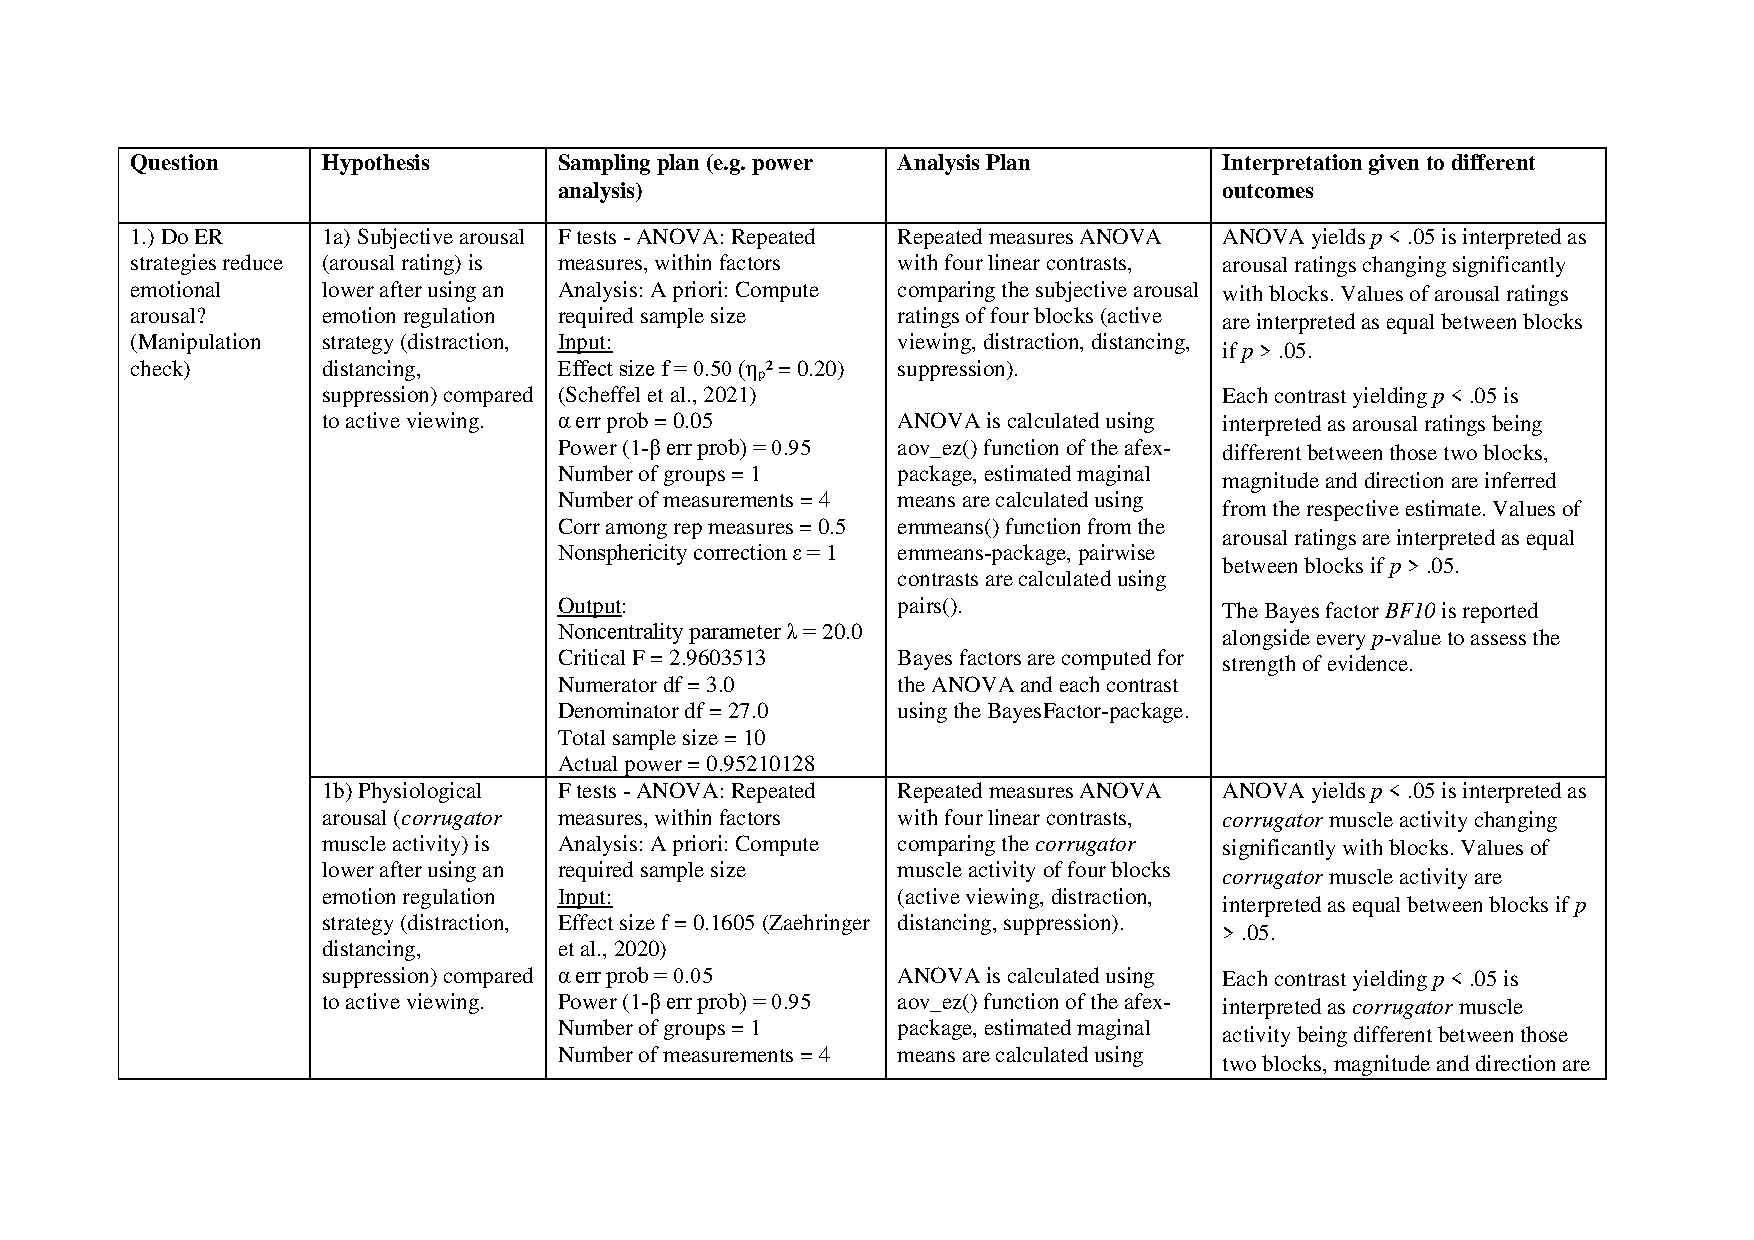
\includepdf[pages={-}, landscape=true]{Supplement/Design_Table_T2.pdf}

\newpage

\hypertarget{SupplementaryMaterial}{%
\section{Supplementary Material}\label{SupplementaryMaterial}}

INCLUDE SUPPLEMENT HERE


\end{document}
